% !TEX encoding = UTF-8 Unicode
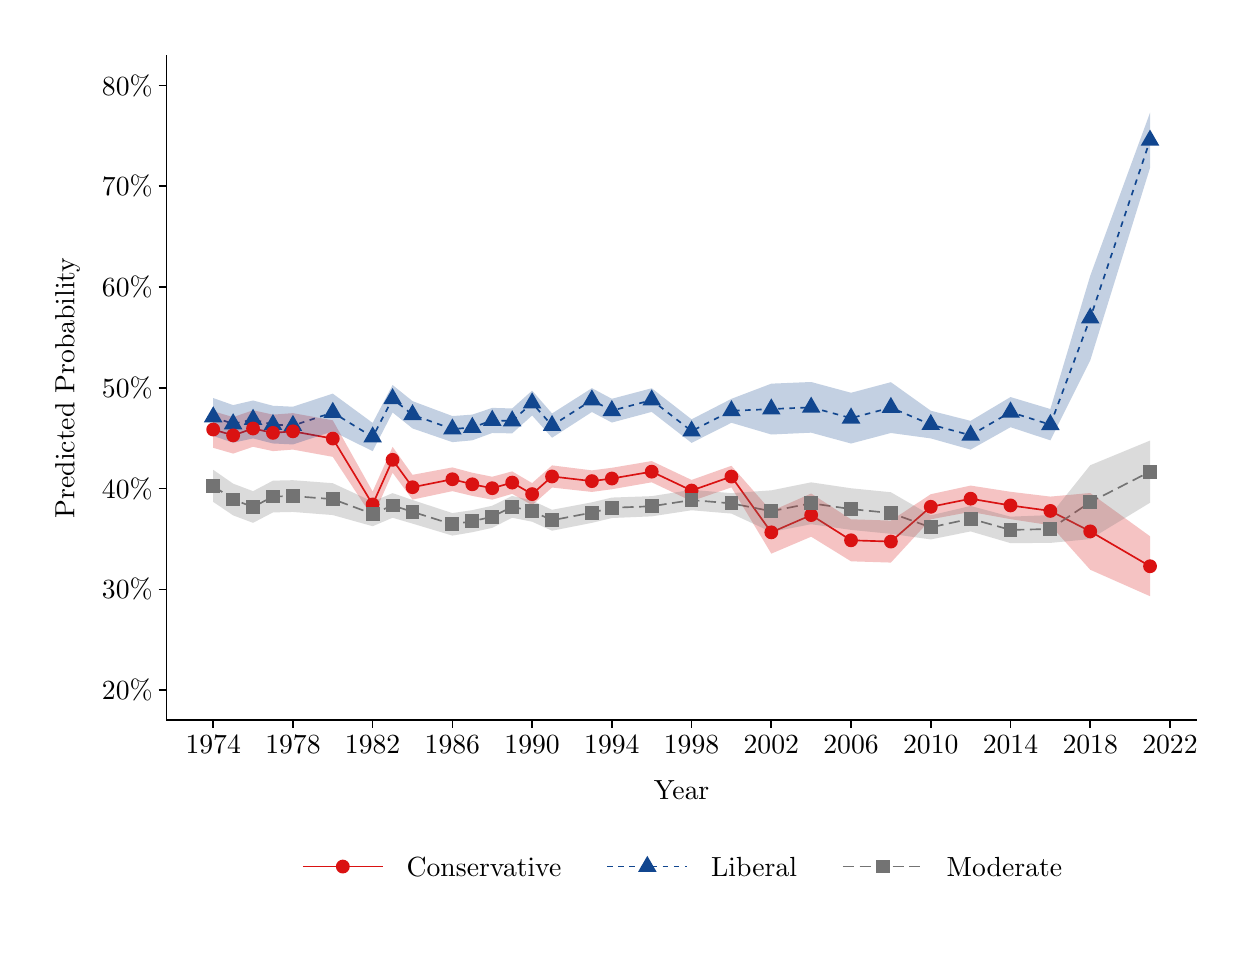
\begin{tikzpicture}[x=1pt,y=1pt]
\definecolor{fillColor}{RGB}{255,255,255}
\path[use as bounding box,fill=fillColor,fill opacity=0.00] (0,0) rectangle (432.48,324.36);
\begin{scope}
\path[clip] (  0.00,  0.00) rectangle (432.48,324.36);
\definecolor{fillColor}{RGB}{255,255,255}

\path[fill=fillColor] ( -0.00,  0.00) rectangle (432.48,324.36);
\end{scope}
\begin{scope}
\path[clip] ( 50.11, 74.07) rectangle (422.48,314.36);
\definecolor{fillColor}{RGB}{255,255,255}

\path[fill=fillColor] ( 50.11, 74.07) rectangle (422.48,314.36);
\definecolor{drawColor}{RGB}{218,18,18}

\path[draw=drawColor,line width= 0.6pt,line join=round] ( 67.04,179.15) --
	( 74.24,177.04) --
	( 81.44,179.51) --
	( 88.64,177.94) --
	( 95.85,178.49) --
	(110.25,175.88) --
	(124.66,152.08) --
	(131.86,168.20) --
	(139.06,158.30) --
	(153.47,161.18) --
	(160.67,159.35) --
	(167.87,157.94) --
	(175.07,159.97) --
	(182.28,155.80) --
	(189.48,162.19) --
	(203.88,160.50) --
	(211.09,161.44) --
	(225.49,163.92) --
	(239.90,157.10) --
	(254.30,162.15) --
	(268.71,141.99) --
	(283.11,148.23) --
	(297.52,139.12) --
	(311.92,138.66) --
	(326.33,151.23) --
	(340.73,154.15) --
	(355.14,151.71) --
	(369.54,149.74) --
	(383.95,142.34) --
	(405.56,129.74);
\definecolor{drawColor}{RGB}{17,70,143}

\path[draw=drawColor,line width= 0.6pt,dash pattern=on 2pt off 2pt ,line join=round] ( 67.04,183.69) --
	( 74.24,181.18) --
	( 81.44,182.79) --
	( 88.64,180.92) --
	( 95.85,180.58) --
	(110.25,185.30) --
	(124.66,176.44) --
	(131.86,190.27) --
	(139.06,184.48) --
	(153.47,179.31) --
	(160.67,179.89) --
	(167.87,182.43) --
	(175.07,182.26) --
	(182.28,188.72) --
	(189.48,180.57) --
	(203.88,189.79) --
	(211.09,185.96) --
	(225.49,189.79) --
	(239.90,178.58) --
	(254.30,185.91) --
	(268.71,186.54) --
	(283.11,187.17) --
	(297.52,183.26) --
	(311.92,187.07) --
	(326.33,180.94) --
	(340.73,177.08) --
	(355.14,185.43) --
	(369.54,180.90) --
	(383.95,219.41) --
	(405.56,283.66);
\definecolor{drawColor}{gray}{0.45}

\path[draw=drawColor,line width= 0.6pt,dash pattern=on 4pt off 2pt ,line join=round] ( 67.04,158.79) --
	( 74.24,153.86) --
	( 81.44,151.15) --
	( 88.64,154.93) --
	( 95.85,155.10) --
	(110.25,153.99) --
	(124.66,148.65) --
	(131.86,151.72) --
	(139.06,149.41) --
	(153.47,144.88) --
	(160.67,146.03) --
	(167.87,147.61) --
	(175.07,151.22) --
	(182.28,149.67) --
	(189.48,146.36) --
	(203.88,149.13) --
	(211.09,150.86) --
	(225.49,151.42) --
	(239.90,153.66) --
	(254.30,152.46) --
	(268.71,149.64) --
	(283.11,152.50) --
	(297.52,150.40) --
	(311.92,148.97) --
	(326.33,143.79) --
	(340.73,146.93) --
	(355.14,142.88) --
	(369.54,143.20) --
	(383.95,152.91) --
	(405.56,163.92);
\definecolor{fillColor}{RGB}{218,18,18}

\path[fill=fillColor,fill opacity=0.25] ( 67.04,185.77) --
	( 74.24,183.63) --
	( 81.44,186.11) --
	( 88.64,184.53) --
	( 95.85,185.07) --
	(110.25,182.47) --
	(124.66,156.74) --
	(131.86,172.87) --
	(139.06,162.77) --
	(153.47,165.46) --
	(160.67,163.54) --
	(167.87,162.08) --
	(175.07,164.02) --
	(182.28,159.79) --
	(189.48,166.19) --
	(203.88,164.39) --
	(211.09,165.32) --
	(225.49,167.75) --
	(239.90,160.93) --
	(254.30,166.05) --
	(268.71,149.67) --
	(283.11,156.03) --
	(297.52,146.71) --
	(311.92,146.24) --
	(326.33,155.77) --
	(340.73,158.89) --
	(355.14,156.65) --
	(369.54,154.91) --
	(383.95,156.21) --
	(405.56,140.57) --
	(405.56,118.92) --
	(383.95,128.48) --
	(369.54,144.57) --
	(355.14,146.76) --
	(340.73,149.40) --
	(326.33,146.70) --
	(311.92,131.07) --
	(297.52,131.53) --
	(283.11,140.42) --
	(268.71,134.30) --
	(254.30,158.25) --
	(239.90,153.27) --
	(225.49,160.08) --
	(211.09,157.57) --
	(203.88,156.60) --
	(189.48,158.19) --
	(182.28,151.80) --
	(175.07,155.91) --
	(167.87,153.80) --
	(160.67,155.16) --
	(153.47,156.89) --
	(139.06,153.83) --
	(131.86,163.53) --
	(124.66,147.42) --
	(110.25,169.28) --
	( 95.85,171.90) --
	( 88.64,171.35) --
	( 81.44,172.91) --
	( 74.24,170.46) --
	( 67.04,172.54) --
	cycle;

\path[] ( 67.04,185.77) --
	( 74.24,183.63) --
	( 81.44,186.11) --
	( 88.64,184.53) --
	( 95.85,185.07) --
	(110.25,182.47) --
	(124.66,156.74) --
	(131.86,172.87) --
	(139.06,162.77) --
	(153.47,165.46) --
	(160.67,163.54) --
	(167.87,162.08) --
	(175.07,164.02) --
	(182.28,159.79) --
	(189.48,166.19) --
	(203.88,164.39) --
	(211.09,165.32) --
	(225.49,167.75) --
	(239.90,160.93) --
	(254.30,166.05) --
	(268.71,149.67) --
	(283.11,156.03) --
	(297.52,146.71) --
	(311.92,146.24) --
	(326.33,155.77) --
	(340.73,158.89) --
	(355.14,156.65) --
	(369.54,154.91) --
	(383.95,156.21) --
	(405.56,140.57);

\path[] (405.56,118.92) --
	(383.95,128.48) --
	(369.54,144.57) --
	(355.14,146.76) --
	(340.73,149.40) --
	(326.33,146.70) --
	(311.92,131.07) --
	(297.52,131.53) --
	(283.11,140.42) --
	(268.71,134.30) --
	(254.30,158.25) --
	(239.90,153.27) --
	(225.49,160.08) --
	(211.09,157.57) --
	(203.88,156.60) --
	(189.48,158.19) --
	(182.28,151.80) --
	(175.07,155.91) --
	(167.87,153.80) --
	(160.67,155.16) --
	(153.47,156.89) --
	(139.06,153.83) --
	(131.86,163.53) --
	(124.66,147.42) --
	(110.25,169.28) --
	( 95.85,171.90) --
	( 88.64,171.35) --
	( 81.44,172.91) --
	( 74.24,170.46) --
	( 67.04,172.54);
\definecolor{fillColor}{RGB}{17,70,143}

\path[fill=fillColor,fill opacity=0.25] ( 67.04,190.52) --
	( 74.24,187.97) --
	( 81.44,189.64) --
	( 88.64,187.73) --
	( 95.85,187.39) --
	(110.25,192.12) --
	(124.66,181.54) --
	(131.86,195.22) --
	(139.06,189.41) --
	(153.47,184.02) --
	(160.67,184.53) --
	(167.87,186.97) --
	(175.07,186.76) --
	(182.28,193.21) --
	(189.48,184.95) --
	(203.88,194.10) --
	(211.09,190.25) --
	(225.49,194.06) --
	(239.90,182.83) --
	(254.30,190.24) --
	(268.71,195.72) --
	(283.11,196.32) --
	(297.52,192.43) --
	(311.92,196.25) --
	(326.33,185.94) --
	(340.73,182.28) --
	(355.14,190.88) --
	(369.54,186.56) --
	(383.95,234.72) --
	(405.56,293.63) --
	(405.56,273.70) --
	(383.95,204.11) --
	(369.54,175.25) --
	(355.14,179.99) --
	(340.73,171.89) --
	(326.33,175.94) --
	(311.92,177.90) --
	(297.52,174.09) --
	(283.11,178.01) --
	(268.71,177.35) --
	(254.30,181.59) --
	(239.90,174.32) --
	(225.49,185.52) --
	(211.09,181.67) --
	(203.88,185.48) --
	(189.48,176.18) --
	(182.28,184.22) --
	(175.07,177.76) --
	(167.87,177.90) --
	(160.67,175.25) --
	(153.47,174.59) --
	(139.06,179.55) --
	(131.86,185.32) --
	(124.66,171.33) --
	(110.25,178.48) --
	( 95.85,173.76) --
	( 88.64,174.11) --
	( 81.44,175.93) --
	( 74.24,174.38) --
	( 67.04,176.85) --
	cycle;

\path[] ( 67.04,190.52) --
	( 74.24,187.97) --
	( 81.44,189.64) --
	( 88.64,187.73) --
	( 95.85,187.39) --
	(110.25,192.12) --
	(124.66,181.54) --
	(131.86,195.22) --
	(139.06,189.41) --
	(153.47,184.02) --
	(160.67,184.53) --
	(167.87,186.97) --
	(175.07,186.76) --
	(182.28,193.21) --
	(189.48,184.95) --
	(203.88,194.10) --
	(211.09,190.25) --
	(225.49,194.06) --
	(239.90,182.83) --
	(254.30,190.24) --
	(268.71,195.72) --
	(283.11,196.32) --
	(297.52,192.43) --
	(311.92,196.25) --
	(326.33,185.94) --
	(340.73,182.28) --
	(355.14,190.88) --
	(369.54,186.56) --
	(383.95,234.72) --
	(405.56,293.63);

\path[] (405.56,273.70) --
	(383.95,204.11) --
	(369.54,175.25) --
	(355.14,179.99) --
	(340.73,171.89) --
	(326.33,175.94) --
	(311.92,177.90) --
	(297.52,174.09) --
	(283.11,178.01) --
	(268.71,177.35) --
	(254.30,181.59) --
	(239.90,174.32) --
	(225.49,185.52) --
	(211.09,181.67) --
	(203.88,185.48) --
	(189.48,176.18) --
	(182.28,184.22) --
	(175.07,177.76) --
	(167.87,177.90) --
	(160.67,175.25) --
	(153.47,174.59) --
	(139.06,179.55) --
	(131.86,185.32) --
	(124.66,171.33) --
	(110.25,178.48) --
	( 95.85,173.76) --
	( 88.64,174.11) --
	( 81.44,175.93) --
	( 74.24,174.38) --
	( 67.04,176.85);
\definecolor{fillColor}{RGB}{115,115,115}

\path[fill=fillColor,fill opacity=0.25] ( 67.04,164.59) --
	( 74.24,159.59) --
	( 81.44,156.87) --
	( 88.64,160.67) --
	( 95.85,160.84) --
	(110.25,159.75) --
	(124.66,153.09) --
	(131.86,156.17) --
	(139.06,153.68) --
	(153.47,148.95) --
	(160.67,150.02) --
	(167.87,151.61) --
	(175.07,155.16) --
	(182.28,153.49) --
	(189.48,150.14) --
	(203.88,152.84) --
	(211.09,154.56) --
	(225.49,155.07) --
	(239.90,157.35) --
	(254.30,156.16) --
	(268.71,157.17) --
	(283.11,160.06) --
	(297.52,157.92) --
	(311.92,156.48) --
	(326.33,148.14) --
	(340.73,151.53) --
	(355.14,147.66) --
	(369.54,148.22) --
	(383.95,166.24) --
	(405.56,175.15) --
	(405.56,152.69) --
	(383.95,139.57) --
	(369.54,138.18) --
	(355.14,138.10) --
	(340.73,142.33) --
	(326.33,139.44) --
	(311.92,141.46) --
	(297.52,142.88) --
	(283.11,144.93) --
	(268.71,142.12) --
	(254.30,148.77) --
	(239.90,149.98) --
	(225.49,147.77) --
	(211.09,147.17) --
	(203.88,145.42) --
	(189.48,142.58) --
	(182.28,145.85) --
	(175.07,147.29) --
	(167.87,143.62) --
	(160.67,142.04) --
	(153.47,140.82) --
	(139.06,145.15) --
	(131.86,147.27) --
	(124.66,144.21) --
	(110.25,148.24) --
	( 95.85,149.36) --
	( 88.64,149.20) --
	( 81.44,145.43) --
	( 74.24,148.13) --
	( 67.04,153.00) --
	cycle;

\path[] ( 67.04,164.59) --
	( 74.24,159.59) --
	( 81.44,156.87) --
	( 88.64,160.67) --
	( 95.85,160.84) --
	(110.25,159.75) --
	(124.66,153.09) --
	(131.86,156.17) --
	(139.06,153.68) --
	(153.47,148.95) --
	(160.67,150.02) --
	(167.87,151.61) --
	(175.07,155.16) --
	(182.28,153.49) --
	(189.48,150.14) --
	(203.88,152.84) --
	(211.09,154.56) --
	(225.49,155.07) --
	(239.90,157.35) --
	(254.30,156.16) --
	(268.71,157.17) --
	(283.11,160.06) --
	(297.52,157.92) --
	(311.92,156.48) --
	(326.33,148.14) --
	(340.73,151.53) --
	(355.14,147.66) --
	(369.54,148.22) --
	(383.95,166.24) --
	(405.56,175.15);

\path[] (405.56,152.69) --
	(383.95,139.57) --
	(369.54,138.18) --
	(355.14,138.10) --
	(340.73,142.33) --
	(326.33,139.44) --
	(311.92,141.46) --
	(297.52,142.88) --
	(283.11,144.93) --
	(268.71,142.12) --
	(254.30,148.77) --
	(239.90,149.98) --
	(225.49,147.77) --
	(211.09,147.17) --
	(203.88,145.42) --
	(189.48,142.58) --
	(182.28,145.85) --
	(175.07,147.29) --
	(167.87,143.62) --
	(160.67,142.04) --
	(153.47,140.82) --
	(139.06,145.15) --
	(131.86,147.27) --
	(124.66,144.21) --
	(110.25,148.24) --
	( 95.85,149.36) --
	( 88.64,149.20) --
	( 81.44,145.43) --
	( 74.24,148.13) --
	( 67.04,153.00);
\definecolor{fillColor}{RGB}{17,70,143}

\path[fill=fillColor] ( 67.04,187.57) --
	( 70.40,181.75) --
	( 63.67,181.75) --
	cycle;

\path[fill=fillColor] ( 74.24,185.06) --
	( 77.60,179.23) --
	( 70.87,179.23) --
	cycle;

\path[fill=fillColor] ( 81.44,186.67) --
	( 84.80,180.84) --
	( 78.08,180.84) --
	cycle;

\path[fill=fillColor] ( 88.64,184.80) --
	( 92.01,178.98) --
	( 85.28,178.98) --
	cycle;

\path[fill=fillColor] ( 95.85,184.46) --
	( 99.21,178.63) --
	( 92.48,178.63) --
	cycle;

\path[fill=fillColor] (110.25,189.18) --
	(113.62,183.36) --
	(106.89,183.36) --
	cycle;

\path[fill=fillColor] (124.66,180.32) --
	(128.02,174.49) --
	(121.29,174.49) --
	cycle;

\path[fill=fillColor] (131.86,194.15) --
	(135.22,188.32) --
	(128.50,188.32) --
	cycle;

\path[fill=fillColor] (139.06,188.37) --
	(142.43,182.54) --
	(135.70,182.54) --
	cycle;

\path[fill=fillColor] (153.47,183.19) --
	(156.83,177.36) --
	(150.10,177.36) --
	cycle;

\path[fill=fillColor] (160.67,183.77) --
	(164.03,177.95) --
	(157.31,177.95) --
	cycle;

\path[fill=fillColor] (167.87,186.32) --
	(171.24,180.49) --
	(164.51,180.49) --
	cycle;

\path[fill=fillColor] (175.07,186.14) --
	(178.44,180.31) --
	(171.71,180.31) --
	cycle;

\path[fill=fillColor] (182.28,192.60) --
	(185.64,186.77) --
	(178.91,186.77) --
	cycle;

\path[fill=fillColor] (189.48,184.45) --
	(192.84,178.63) --
	(186.12,178.63) --
	cycle;

\path[fill=fillColor] (203.88,193.67) --
	(207.25,187.84) --
	(200.52,187.84) --
	cycle;

\path[fill=fillColor] (211.09,189.84) --
	(214.45,184.02) --
	(207.72,184.02) --
	cycle;

\path[fill=fillColor] (225.49,193.67) --
	(228.86,187.85) --
	(222.13,187.85) --
	cycle;

\path[fill=fillColor] (239.90,182.46) --
	(243.26,176.64) --
	(236.53,176.64) --
	cycle;

\path[fill=fillColor] (254.30,189.80) --
	(257.67,183.97) --
	(250.94,183.97) --
	cycle;

\path[fill=fillColor] (268.71,190.42) --
	(272.07,184.59) --
	(265.34,184.59) --
	cycle;

\path[fill=fillColor] (283.11,191.05) --
	(286.48,185.22) --
	(279.75,185.22) --
	cycle;

\path[fill=fillColor] (297.52,187.15) --
	(300.88,181.32) --
	(294.15,181.32) --
	cycle;

\path[fill=fillColor] (311.92,190.96) --
	(315.29,185.13) --
	(308.56,185.13) --
	cycle;

\path[fill=fillColor] (326.33,184.83) --
	(329.69,179.00) --
	(322.96,179.00) --
	cycle;

\path[fill=fillColor] (340.73,180.97) --
	(344.10,175.14) --
	(337.37,175.14) --
	cycle;

\path[fill=fillColor] (355.14,189.32) --
	(358.50,183.49) --
	(351.77,183.49) --
	cycle;

\path[fill=fillColor] (369.54,184.79) --
	(372.91,178.96) --
	(366.18,178.96) --
	cycle;

\path[fill=fillColor] (383.95,223.30) --
	(387.31,217.47) --
	(380.58,217.47) --
	cycle;

\path[fill=fillColor] (405.56,287.55) --
	(408.92,281.72) --
	(402.19,281.72) --
	cycle;
\definecolor{fillColor}{RGB}{218,18,18}

\path[fill=fillColor] ( 67.04,179.15) circle (  2.50);

\path[fill=fillColor] ( 74.24,177.04) circle (  2.50);

\path[fill=fillColor] ( 81.44,179.51) circle (  2.50);

\path[fill=fillColor] ( 88.64,177.94) circle (  2.50);

\path[fill=fillColor] ( 95.85,178.49) circle (  2.50);

\path[fill=fillColor] (110.25,175.88) circle (  2.50);

\path[fill=fillColor] (124.66,152.08) circle (  2.50);

\path[fill=fillColor] (131.86,168.20) circle (  2.50);

\path[fill=fillColor] (139.06,158.30) circle (  2.50);

\path[fill=fillColor] (153.47,161.18) circle (  2.50);

\path[fill=fillColor] (160.67,159.35) circle (  2.50);

\path[fill=fillColor] (167.87,157.94) circle (  2.50);

\path[fill=fillColor] (175.07,159.97) circle (  2.50);

\path[fill=fillColor] (182.28,155.80) circle (  2.50);

\path[fill=fillColor] (189.48,162.19) circle (  2.50);

\path[fill=fillColor] (203.88,160.50) circle (  2.50);

\path[fill=fillColor] (211.09,161.44) circle (  2.50);

\path[fill=fillColor] (225.49,163.92) circle (  2.50);

\path[fill=fillColor] (239.90,157.10) circle (  2.50);

\path[fill=fillColor] (254.30,162.15) circle (  2.50);

\path[fill=fillColor] (268.71,141.99) circle (  2.50);

\path[fill=fillColor] (283.11,148.23) circle (  2.50);

\path[fill=fillColor] (297.52,139.12) circle (  2.50);

\path[fill=fillColor] (311.92,138.66) circle (  2.50);

\path[fill=fillColor] (326.33,151.23) circle (  2.50);

\path[fill=fillColor] (340.73,154.15) circle (  2.50);

\path[fill=fillColor] (355.14,151.71) circle (  2.50);

\path[fill=fillColor] (369.54,149.74) circle (  2.50);

\path[fill=fillColor] (383.95,142.34) circle (  2.50);

\path[fill=fillColor] (405.56,129.74) circle (  2.50);
\definecolor{fillColor}{gray}{0.45}

\path[fill=fillColor] ( 64.54,156.29) --
	( 69.53,156.29) --
	( 69.53,161.29) --
	( 64.54,161.29) --
	cycle;

\path[fill=fillColor] ( 71.74,151.37) --
	( 76.74,151.37) --
	( 76.74,156.36) --
	( 71.74,156.36) --
	cycle;

\path[fill=fillColor] ( 78.94,148.65) --
	( 83.94,148.65) --
	( 83.94,153.65) --
	( 78.94,153.65) --
	cycle;

\path[fill=fillColor] ( 86.15,152.44) --
	( 91.14,152.44) --
	( 91.14,157.43) --
	( 86.15,157.43) --
	cycle;

\path[fill=fillColor] ( 93.35,152.60) --
	( 98.34,152.60) --
	( 98.34,157.60) --
	( 93.35,157.60) --
	cycle;

\path[fill=fillColor] (107.75,151.50) --
	(112.75,151.50) --
	(112.75,156.49) --
	(107.75,156.49) --
	cycle;

\path[fill=fillColor] (122.16,146.15) --
	(127.15,146.15) --
	(127.15,151.15) --
	(122.16,151.15) --
	cycle;

\path[fill=fillColor] (129.36,149.22) --
	(134.36,149.22) --
	(134.36,154.22) --
	(129.36,154.22) --
	cycle;

\path[fill=fillColor] (136.56,146.91) --
	(141.56,146.91) --
	(141.56,151.91) --
	(136.56,151.91) --
	cycle;

\path[fill=fillColor] (150.97,142.39) --
	(155.96,142.39) --
	(155.96,147.38) --
	(150.97,147.38) --
	cycle;

\path[fill=fillColor] (158.17,143.53) --
	(163.17,143.53) --
	(163.17,148.53) --
	(158.17,148.53) --
	cycle;

\path[fill=fillColor] (165.37,145.11) --
	(170.37,145.11) --
	(170.37,150.11) --
	(165.37,150.11) --
	cycle;

\path[fill=fillColor] (172.58,148.73) --
	(177.57,148.73) --
	(177.57,153.72) --
	(172.58,153.72) --
	cycle;

\path[fill=fillColor] (179.78,147.17) --
	(184.77,147.17) --
	(184.77,152.17) --
	(179.78,152.17) --
	cycle;

\path[fill=fillColor] (186.98,143.86) --
	(191.98,143.86) --
	(191.98,148.86) --
	(186.98,148.86) --
	cycle;

\path[fill=fillColor] (201.39,146.63) --
	(206.38,146.63) --
	(206.38,151.62) --
	(201.39,151.62) --
	cycle;

\path[fill=fillColor] (208.59,148.36) --
	(213.58,148.36) --
	(213.58,153.36) --
	(208.59,153.36) --
	cycle;

\path[fill=fillColor] (222.99,148.92) --
	(227.99,148.92) --
	(227.99,153.92) --
	(222.99,153.92) --
	cycle;

\path[fill=fillColor] (237.40,151.17) --
	(242.39,151.17) --
	(242.39,156.16) --
	(237.40,156.16) --
	cycle;

\path[fill=fillColor] (251.80,149.97) --
	(256.80,149.97) --
	(256.80,154.96) --
	(251.80,154.96) --
	cycle;

\path[fill=fillColor] (266.21,147.15) --
	(271.21,147.15) --
	(271.21,152.14) --
	(266.21,152.14) --
	cycle;

\path[fill=fillColor] (280.61,150.00) --
	(285.61,150.00) --
	(285.61,154.99) --
	(280.61,154.99) --
	cycle;

\path[fill=fillColor] (295.02,147.91) --
	(300.02,147.91) --
	(300.02,152.90) --
	(295.02,152.90) --
	cycle;

\path[fill=fillColor] (309.43,146.47) --
	(314.42,146.47) --
	(314.42,151.47) --
	(309.43,151.47) --
	cycle;

\path[fill=fillColor] (323.83,141.29) --
	(328.83,141.29) --
	(328.83,146.29) --
	(323.83,146.29) --
	cycle;

\path[fill=fillColor] (338.24,144.43) --
	(343.23,144.43) --
	(343.23,149.43) --
	(338.24,149.43) --
	cycle;

\path[fill=fillColor] (352.64,140.38) --
	(357.64,140.38) --
	(357.64,145.38) --
	(352.64,145.38) --
	cycle;

\path[fill=fillColor] (367.05,140.70) --
	(372.04,140.70) --
	(372.04,145.70) --
	(367.05,145.70) --
	cycle;

\path[fill=fillColor] (381.45,150.41) --
	(386.45,150.41) --
	(386.45,155.41) --
	(381.45,155.41) --
	cycle;

\path[fill=fillColor] (403.06,161.42) --
	(408.05,161.42) --
	(408.05,166.42) --
	(403.06,166.42) --
	cycle;
\end{scope}
\begin{scope}
\path[clip] (  0.00,  0.00) rectangle (432.48,324.36);
\definecolor{drawColor}{RGB}{0,0,0}

\path[draw=drawColor,line width= 0.6pt,line join=round] ( 50.11, 74.07) --
	( 50.11,314.36);
\end{scope}
\begin{scope}
\path[clip] (  0.00,  0.00) rectangle (432.48,324.36);
\definecolor{drawColor}{RGB}{0,0,0}

\node[text=drawColor,anchor=base east,inner sep=0pt, outer sep=0pt, scale=  1.00] at ( 45.16, 81.55) {20{\%}};

\node[text=drawColor,anchor=base east,inner sep=0pt, outer sep=0pt, scale=  1.00] at ( 45.16,117.95) {30{\%}};

\node[text=drawColor,anchor=base east,inner sep=0pt, outer sep=0pt, scale=  1.00] at ( 45.16,154.36) {40{\%}};

\node[text=drawColor,anchor=base east,inner sep=0pt, outer sep=0pt, scale=  1.00] at ( 45.16,190.77) {50{\%}};

\node[text=drawColor,anchor=base east,inner sep=0pt, outer sep=0pt, scale=  1.00] at ( 45.16,227.18) {60{\%}};

\node[text=drawColor,anchor=base east,inner sep=0pt, outer sep=0pt, scale=  1.00] at ( 45.16,263.59) {70{\%}};

\node[text=drawColor,anchor=base east,inner sep=0pt, outer sep=0pt, scale=  1.00] at ( 45.16,300.00) {80{\%}};
\end{scope}
\begin{scope}
\path[clip] (  0.00,  0.00) rectangle (432.48,324.36);
\definecolor{drawColor}{RGB}{0,0,0}

\path[draw=drawColor,line width= 0.6pt,line join=round] ( 47.36, 84.99) --
	( 50.11, 84.99);

\path[draw=drawColor,line width= 0.6pt,line join=round] ( 47.36,121.40) --
	( 50.11,121.40);

\path[draw=drawColor,line width= 0.6pt,line join=round] ( 47.36,157.81) --
	( 50.11,157.81);

\path[draw=drawColor,line width= 0.6pt,line join=round] ( 47.36,194.21) --
	( 50.11,194.21);

\path[draw=drawColor,line width= 0.6pt,line join=round] ( 47.36,230.62) --
	( 50.11,230.62);

\path[draw=drawColor,line width= 0.6pt,line join=round] ( 47.36,267.03) --
	( 50.11,267.03);

\path[draw=drawColor,line width= 0.6pt,line join=round] ( 47.36,303.44) --
	( 50.11,303.44);
\end{scope}
\begin{scope}
\path[clip] (  0.00,  0.00) rectangle (432.48,324.36);
\definecolor{drawColor}{RGB}{0,0,0}

\path[draw=drawColor,line width= 0.6pt,line join=round] ( 50.11, 74.07) --
	(422.48, 74.07);
\end{scope}
\begin{scope}
\path[clip] (  0.00,  0.00) rectangle (432.48,324.36);
\definecolor{drawColor}{RGB}{0,0,0}

\path[draw=drawColor,line width= 0.6pt,line join=round] ( 67.04, 71.32) --
	( 67.04, 74.07);

\path[draw=drawColor,line width= 0.6pt,line join=round] ( 95.85, 71.32) --
	( 95.85, 74.07);

\path[draw=drawColor,line width= 0.6pt,line join=round] (124.66, 71.32) --
	(124.66, 74.07);

\path[draw=drawColor,line width= 0.6pt,line join=round] (153.47, 71.32) --
	(153.47, 74.07);

\path[draw=drawColor,line width= 0.6pt,line join=round] (182.28, 71.32) --
	(182.28, 74.07);

\path[draw=drawColor,line width= 0.6pt,line join=round] (211.09, 71.32) --
	(211.09, 74.07);

\path[draw=drawColor,line width= 0.6pt,line join=round] (239.90, 71.32) --
	(239.90, 74.07);

\path[draw=drawColor,line width= 0.6pt,line join=round] (268.71, 71.32) --
	(268.71, 74.07);

\path[draw=drawColor,line width= 0.6pt,line join=round] (297.52, 71.32) --
	(297.52, 74.07);

\path[draw=drawColor,line width= 0.6pt,line join=round] (326.33, 71.32) --
	(326.33, 74.07);

\path[draw=drawColor,line width= 0.6pt,line join=round] (355.14, 71.32) --
	(355.14, 74.07);

\path[draw=drawColor,line width= 0.6pt,line join=round] (383.95, 71.32) --
	(383.95, 74.07);

\path[draw=drawColor,line width= 0.6pt,line join=round] (412.76, 71.32) --
	(412.76, 74.07);
\end{scope}
\begin{scope}
\path[clip] (  0.00,  0.00) rectangle (432.48,324.36);
\definecolor{drawColor}{RGB}{0,0,0}

\node[text=drawColor,anchor=base,inner sep=0pt, outer sep=0pt, scale=  1.00] at ( 67.04, 62.23) {1974};

\node[text=drawColor,anchor=base,inner sep=0pt, outer sep=0pt, scale=  1.00] at ( 95.85, 62.23) {1978};

\node[text=drawColor,anchor=base,inner sep=0pt, outer sep=0pt, scale=  1.00] at (124.66, 62.23) {1982};

\node[text=drawColor,anchor=base,inner sep=0pt, outer sep=0pt, scale=  1.00] at (153.47, 62.23) {1986};

\node[text=drawColor,anchor=base,inner sep=0pt, outer sep=0pt, scale=  1.00] at (182.28, 62.23) {1990};

\node[text=drawColor,anchor=base,inner sep=0pt, outer sep=0pt, scale=  1.00] at (211.09, 62.23) {1994};

\node[text=drawColor,anchor=base,inner sep=0pt, outer sep=0pt, scale=  1.00] at (239.90, 62.23) {1998};

\node[text=drawColor,anchor=base,inner sep=0pt, outer sep=0pt, scale=  1.00] at (268.71, 62.23) {2002};

\node[text=drawColor,anchor=base,inner sep=0pt, outer sep=0pt, scale=  1.00] at (297.52, 62.23) {2006};

\node[text=drawColor,anchor=base,inner sep=0pt, outer sep=0pt, scale=  1.00] at (326.33, 62.23) {2010};

\node[text=drawColor,anchor=base,inner sep=0pt, outer sep=0pt, scale=  1.00] at (355.14, 62.23) {2014};

\node[text=drawColor,anchor=base,inner sep=0pt, outer sep=0pt, scale=  1.00] at (383.95, 62.23) {2018};

\node[text=drawColor,anchor=base,inner sep=0pt, outer sep=0pt, scale=  1.00] at (412.76, 62.23) {2022};
\end{scope}
\begin{scope}
\path[clip] (  0.00,  0.00) rectangle (432.48,324.36);
\definecolor{drawColor}{RGB}{0,0,0}

\node[text=drawColor,anchor=base,inner sep=0pt, outer sep=0pt, scale=  1.00] at (236.30, 45.40) {Year};
\end{scope}
\begin{scope}
\path[clip] (  0.00,  0.00) rectangle (432.48,324.36);
\definecolor{drawColor}{RGB}{0,0,0}

\node[text=drawColor,rotate= 90.00,anchor=base,inner sep=0pt, outer sep=0pt, scale=  1.00] at ( 16.89,194.21) {Predicted Probability};
\end{scope}
\begin{scope}
\path[clip] (  0.00,  0.00) rectangle (432.48,324.36);

\path[] ( 86.80, 10.00) rectangle (385.79, 32.45);
\end{scope}
\begin{scope}
\path[clip] (  0.00,  0.00) rectangle (432.48,324.36);

\path[] ( 95.80, 14.00) rectangle (131.94, 28.45);
\end{scope}
\begin{scope}
\path[clip] (  0.00,  0.00) rectangle (432.48,324.36);
\definecolor{drawColor}{RGB}{218,18,18}

\path[draw=drawColor,line width= 0.6pt,line join=round] ( 99.42, 21.23) -- (128.33, 21.23);
\end{scope}
\begin{scope}
\path[clip] (  0.00,  0.00) rectangle (432.48,324.36);
\definecolor{fillColor}{RGB}{218,18,18}

\path[fill=fillColor] (113.87, 21.23) circle (  2.50);
\end{scope}
\begin{scope}
\path[clip] (  0.00,  0.00) rectangle (432.48,324.36);

\path[] (205.84, 14.00) rectangle (241.98, 28.45);
\end{scope}
\begin{scope}
\path[clip] (  0.00,  0.00) rectangle (432.48,324.36);
\definecolor{drawColor}{RGB}{17,70,143}

\path[draw=drawColor,line width= 0.6pt,dash pattern=on 2pt off 2pt ,line join=round] (209.46, 21.23) -- (238.36, 21.23);
\end{scope}
\begin{scope}
\path[clip] (  0.00,  0.00) rectangle (432.48,324.36);
\definecolor{fillColor}{RGB}{17,70,143}

\path[fill=fillColor] (223.91, 25.11) --
	(227.27, 19.28) --
	(220.55, 19.28) --
	cycle;
\end{scope}
\begin{scope}
\path[clip] (  0.00,  0.00) rectangle (432.48,324.36);

\path[] (290.97, 14.00) rectangle (327.10, 28.45);
\end{scope}
\begin{scope}
\path[clip] (  0.00,  0.00) rectangle (432.48,324.36);
\definecolor{drawColor}{gray}{0.45}

\path[draw=drawColor,line width= 0.6pt,dash pattern=on 4pt off 2pt ,line join=round] (294.58, 21.23) -- (323.49, 21.23);
\end{scope}
\begin{scope}
\path[clip] (  0.00,  0.00) rectangle (432.48,324.36);
\definecolor{fillColor}{gray}{0.45}

\path[fill=fillColor] (306.54, 18.73) --
	(311.53, 18.73) --
	(311.53, 23.72) --
	(306.54, 23.72) --
	cycle;
\end{scope}
\begin{scope}
\path[clip] (  0.00,  0.00) rectangle (432.48,324.36);
\definecolor{drawColor}{RGB}{0,0,0}

\node[text=drawColor,anchor=base west,inner sep=0pt, outer sep=0pt, scale=  1.00] at (136.94, 17.78) {Conservative};
\end{scope}
\begin{scope}
\path[clip] (  0.00,  0.00) rectangle (432.48,324.36);
\definecolor{drawColor}{RGB}{0,0,0}

\node[text=drawColor,anchor=base west,inner sep=0pt, outer sep=0pt, scale=  1.00] at (246.98, 17.78) {Liberal};
\end{scope}
\begin{scope}
\path[clip] (  0.00,  0.00) rectangle (432.48,324.36);
\definecolor{drawColor}{RGB}{0,0,0}

\node[text=drawColor,anchor=base west,inner sep=0pt, outer sep=0pt, scale=  1.00] at (332.10, 17.78) {Moderate};
\end{scope}
\end{tikzpicture}
